\chapter{РУКОВОДСТВО ПОЛЬЗОВАТЕЛЯ}

После запуска программы появляется основное окно программы, в соответствии с рисунком \ref{fig:main}. 
%Пользователю доступны следующие действия:
%
%\begin{itemize}
%	\item добавление шаблона;
%	\item редактирование шаблона;
%	\item использование шаблона;
%	\item запуск справки;
%	\item показ информации о программе.
%\end{itemize}

\begin{figure}[ht!]
\centering
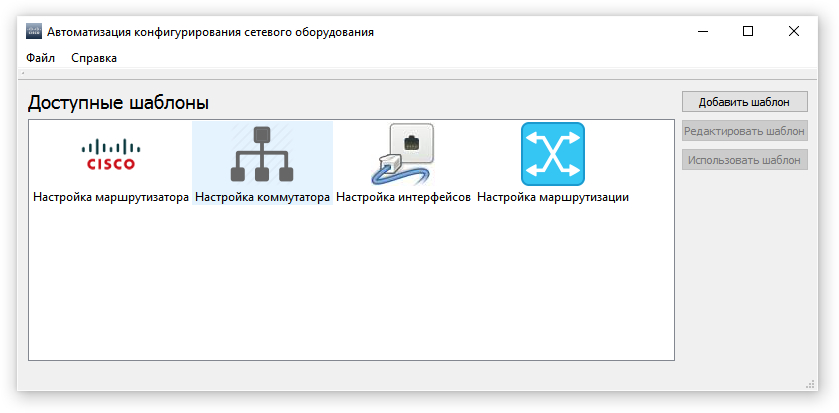
\includegraphics[width=0.8\linewidth]{pic/main}
\caption{Основное окно программы}
\label{fig:main}
\end{figure}

\section{Добавление шаблона}

\label{section:add_template}
\begin{enumerate}
	\item 
Для добавление нового шаблона нажмите кнопку \texttt{<<Добавить шаблон>>}, либо выберите пункт меню \texttt{Файл | Добавить новый шаблон}, либо нажмите сочетание клавиш \texttt{Crtl+N} (в соответствии с рисунком \ref{fig:add_template}).

\begin{figure}[h!]
	\centering
	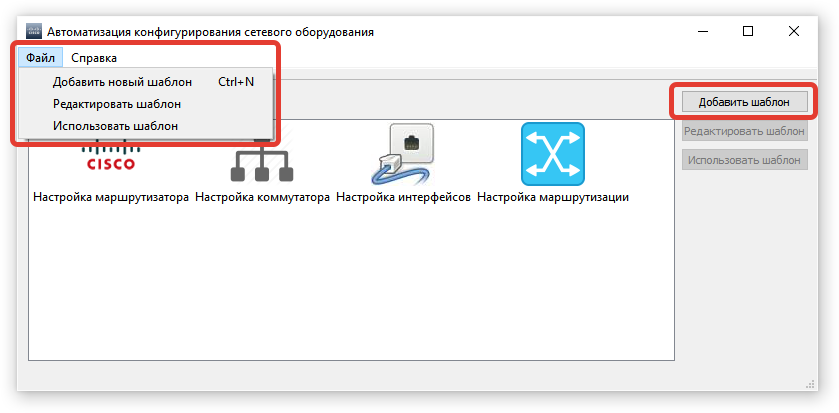
\includegraphics[width=0.8\linewidth]{pic/add_template}
	\caption{Добавление шаблона}
	\label{fig:add_template}
\end{figure}

	\item После этого появится окно добавления нового шаблона (в соответствии с рисунком \ref{fig:template_window}).

\begin{figure}[ht!]
\centering
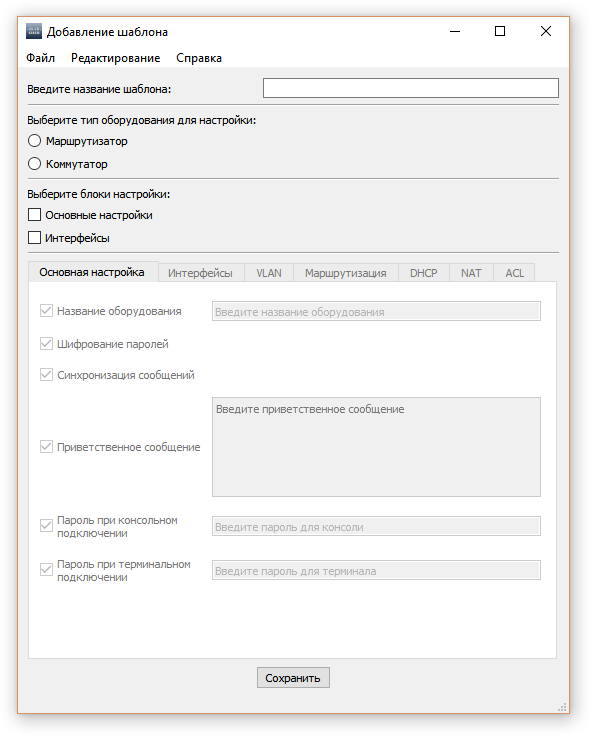
\includegraphics[width=1\linewidth]{pic/template_window}
\caption{Окно добавление шаблона}
\label{fig:template_window}
\end{figure}

	\item Введите название шаблона (в соответствии с рисунком \ref{fig:template_window_edit_name}) для дальнейшей его идентификации в списке других шаблонов.

\begin{figure}[ht!]
\centering
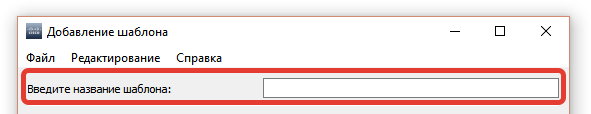
\includegraphics[width=1\linewidth]{pic/template_window_edit_name}
\caption{Ввод названия шаблона}
\label{fig:template_window_edit_name}
\end{figure}

	\item Выберите тип устройства для дальнейших действий (в соответствии с рисунком \ref{fig:template_window_edit_type}).

\begin{figure}[ht!]
\centering
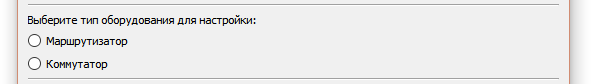
\includegraphics[width=1\linewidth]{pic/template_window_edit_type}
\caption{Выбор типа устройства}
\label{fig:template_window_edit_type}
\end{figure}

Выбор типа <<Маршрутизатор>> позволяет выбирать следующие блоки настройки (в соответствии с рисунком \ref{fig:type_router}):
\begin{itemize}
	\item Основные настройки;
	\item Интерфейсы;
	\item Маршрутизация;
	\item DHCP;
	\item NAT;
	\item ACL.
\end{itemize}

\begin{figure}[th!]
\centering
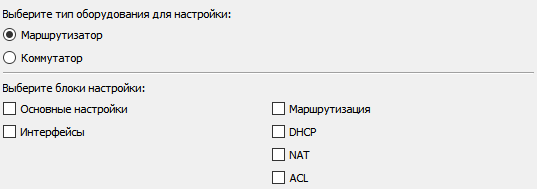
\includegraphics[width=1\linewidth]{pic/type_router}
\caption{Тип <<Маршрутизатор>>}
\label{fig:type_router}
\end{figure}

Выбор типа <<Коммутатор>> позволяет выбирать следующие блоки настройки (в соответствии с рисунком \ref{fig:type_switch}):
\begin{itemize}
	\item Основные настройки;
	\item Интерфейсы;
	\item VLAN.
\end{itemize}

\begin{figure}[th!]
\centering
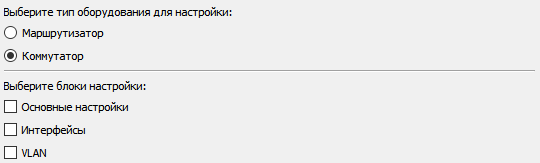
\includegraphics[width=1\linewidth]{pic/type_switch}
\caption{Тип <<Коммутатор>>}
\label{fig:type_switch}
\end{figure}

	\item Выберите блоки настройки из списка в зависимости от необходимого функционала (в соответствии с рисунками \ref{fig:type_router} и \ref{fig:type_switch})
\begin{enumerate}
	\item 	
	При выборе блока <<Основные настройки>> становится доступна доступна страница (в соответствии с рисунком \ref{fig:main_settings}), где можно настроить следующие для добавления в шаблон следующие параметры:
	
	\begin{itemize}
		\item название оборудования;
		\item шифрование паролей;
		\item синхронизация вывода сообщение при наборе команд;
		\item приветственное сообщение;
		\item пароль на консольное подключение;
		\item пароль на терминальное подключение.
	\end{itemize}
	
	По умолчанию, все параметры выбраны. Также можно настроить значения данных параметров по умолчанию.
	
\begin{figure}[th!]
\centering
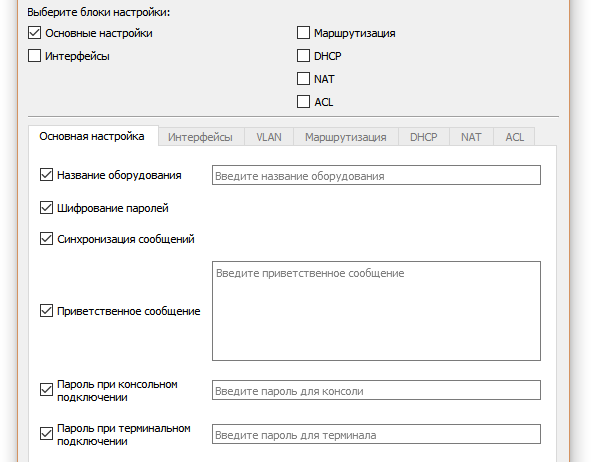
\includegraphics[width=1\linewidth]{pic/main_settings}
\caption{Основные настройки}
\label{fig:main_settings}
\end{figure}

\item 
При выборе блока <<Интерфейсы>> становится доступна страница (в соответствии с рисунком \ref{fig:interface_settings}), где можно добавлять или удалять интерфейсы, необходимые по данному шаблону.
%настроить следующие для добавления в шаблон следующие параметры:
%
%\begin{itemize}
%	\item название оборудования;
%	\item шифрование паролей;
%	\item синхронизация вывода сообщение при наборе команд;
%	\item приветственное сообщение;
%	\item пароль на консольное подключение;
%	\item пароль на терминальное подключение.
%\end{itemize}

\begin{figure}[th!]
\centering
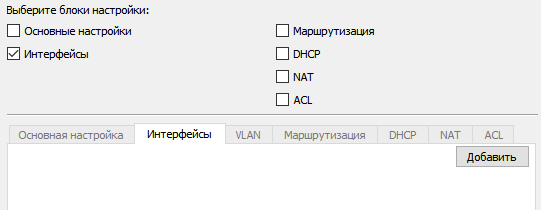
\includegraphics[width=1\linewidth]{pic/interface_settings}
\caption{Интерфейсы}
\label{fig:interface_settings}
\end{figure}

По умолчанию, интерфейсы отсутствуют. Для добавления необходимо нажать кнопку \texttt{<<Добавить>>} либо выбрать пункт меню \texttt{Редактирование | Добавить интерфейс}. 

При добавлении необходимо указать тип интерфейса и его номер. Опционально можно указать описание, режим и скорость передачи данных, IPv4-адрес с маской, IPv6-адрес, а также режим передачи трафика (тегированный или нет) c указанием соответствующих VLAN (в соответствии с рисунком \ref{fig:add_interface}).

\begin{figure}[th!]
	\centering
	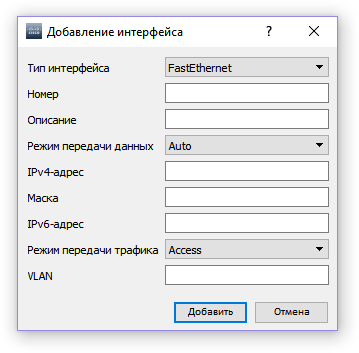
\includegraphics[width=0.8\linewidth]{pic/add_interface}
	\caption{Добавление интерфейса}
	\label{fig:add_interface}
\end{figure}

После нажатия в диалоге кнопки <<Добавить>> в списке интерфейсов появится добавленный интерфейс (в соответствии с рисунком \ref{fig:add_interface_2}).

Для дальнейшего редактирования интерфейса можно дважды кликнуть по названию интерфейса и откроется диалоговое окно, аналогичное окну при добавлении интерфейса. Также присутствует возможность удалить данный интерфейс из шаблона.

%Также можно настроить значения данных параметров по умолчанию.

\begin{figure}[th!]
\centering
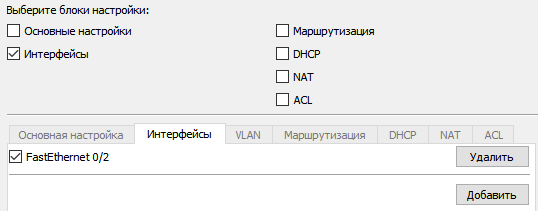
\includegraphics[width=1\linewidth]{pic/add_interface_2}
\caption{Список интерфейсов}
\label{fig:add_interface_2}
\end{figure}

\item 
При выборе блока <<VLAN>> становится доступна страница (в соответствии с рисунком \ref{fig:vlan_settings}), где можно добавлять или удалять VLAN'ы, необходимые по данному шаблону.

\begin{figure}[th!]
	\centering
	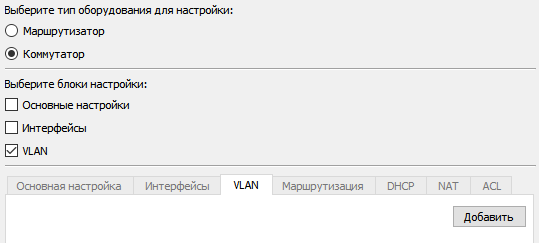
\includegraphics[width=1\linewidth]{pic/vlan_settings}
	\caption{VLAN}
	\label{fig:vlan_settings}
\end{figure}

По умолчанию, интерфейсы отсутствуют. Для добавления необходимо нажать кнопку \texttt{<<Добавить>>} либо выбрать пункт меню \texttt{Редактирование | Добавить VLAN}. 

При добавлении необходимо указать номер VLAN. Опционально можно указать название и описание VLAN. 

\begin{figure}[th!]
	\centering
	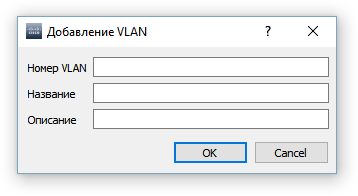
\includegraphics[width=0.8\linewidth]{pic/add_vlan}
	\caption{Добавление VLAN}
	\label{fig:add_vlan}
\end{figure}

После нажатия в диалоге кнопки <<Добавить>> в списке VLAN появится добавленный интерфейс (в соответствии с рисунком \ref{fig:add_vlan_2}).

Для дальнейшего редактирования VLAN можно дважды кликнуть по названию и откроется диалоговое окно, аналогичное окну при добавлении VLAN. Также присутствует возможность удалить данный VLAN из шаблона.

%Также можно настроить значения данных параметров по умолчанию.

\begin{figure}[th!]
	\centering
	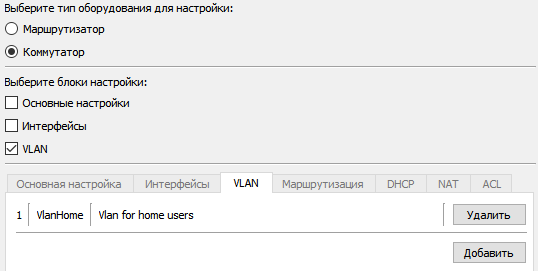
\includegraphics[width=1\linewidth]{pic/add_vlan_2}
	\caption{Список VLAN}
	\label{fig:add_vlan_2}
\end{figure}

\item 
При выборе блока <<Маршрутизация>> становится доступна страница (в соответствии с рисунком \ref{fig:route_settings}), где можно статическую и/или динамическую маршрутизацию.

\begin{figure}[th!]
	\centering
	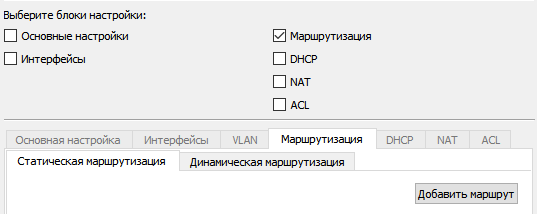
\includegraphics[width=1\linewidth]{pic/route_settings}
	\caption{Маршрутизация}
	\label{fig:route_settings}
\end{figure}

По умолчанию, статические маршруты отсутствуют. Для добавления необходимо нажать кнопку \texttt{<<Добавить>>} во вкладке \texttt{Статическая маршрутизация} либо выбрать пункт меню \texttt{Редактирование | Добавить статический маршрут}. 

При добавлении необходимо указать IP-адрес и маску сети назначения, а также выбрать, через что отправлять пакеты в данную сеть. Можно выбрать либо адрес следующего маршрутизатора с указанием соответствующего IP-адрес, либо интерфейс с указанием соответствующего интерфейса.

\begin{figure}[th!]
	\centering
	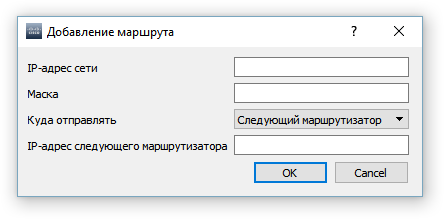
\includegraphics[width=\linewidth]{pic/add_route}
	\caption{Добавление статического маршрута}
	\label{fig:add_route}
\end{figure}

После нажатия в диалоге кнопки <<Добавить>> в списке маршрутов появится добавленный маршрут (в соответствии с рисунком \ref{fig:add_route_2}).

Для дальнейшего редактирования статического маршрута можно дважды кликнуть по названию и откроется диалоговое окно, аналогичное окну при добавлении статического маршрута. Также присутствует возможность удалить данный маршрут из шаблона.

%Также можно настроить значения данных параметров по умолчанию.

\begin{figure}[th!]
	\centering
	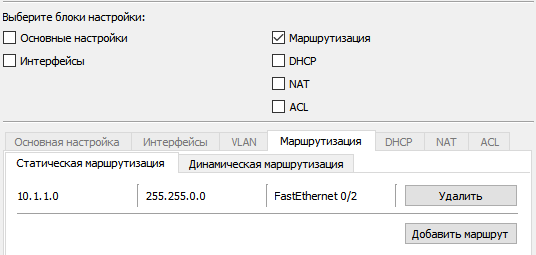
\includegraphics[width=1\linewidth]{pic/add_route_2}
	\caption{Список статических маршрутов}
	\label{fig:add_route_2}
\end{figure}

Для включения команд динамической маршрутизации в шаблон установите пункты OSPF или EIGRP (в соответствии с рисунком \ref{fig:dymanic_route}).

\begin{figure}[th!]
\centering
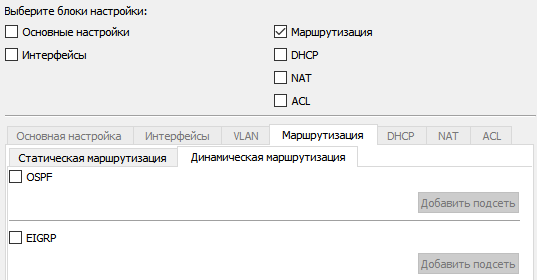
\includegraphics[width=1\linewidth]{pic/dymanic_route}
\caption{Динамическая маршрутизация}
\label{fig:dymanic_route}
\end{figure}

Для добавление сетей в объявления OSPF или EIGRP воспользуйтесь соответствующей кнопкой <<Добавить сеть>> или пунктом меню \texttt{Редактирование | Добавить сеть OSPF} (\texttt{Редактирование | Добавить сеть EIGRP}).

\item 
При выборе блока <<DCHP>> становится доступна страница (в соответствии с рисунком \ref{fig:dhcp_settings}), где можно настроить DHCP.

\begin{figure}[th!]
	\centering
	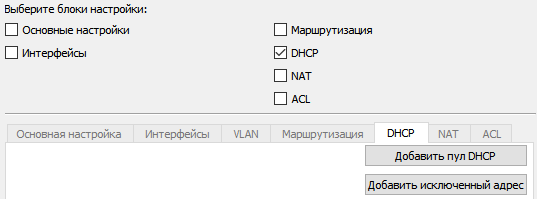
\includegraphics[width=1\linewidth]{pic/dhcp_settings}
	\caption{DHCP}
	\label{fig:dhcp_settings}
\end{figure}

По умолчанию, пулы DHCP отсутствуют. Для добавления пула DHCP, нажмите кнопку \texttt{<<Добавить пул DHCP>>} или выберите пункт меню \texttt{Редактирование | Добавить пул DHCP}. При добавлении необходимо указать IP-адрес сети с маской, а также IP-адрес шлюза. Опционально, можно указать DNS-сервер. После добавления IP-адрес шлюза будет автоматически включен в число исключенных адресов.

 Для добавления исключенного IP-адреса, нажмите кнопку \texttt{<<Добавить исключенный адрес>>} или выберите пункт меню \texttt{Редактирование | Добавить исключенный IP-адрес}.

\item 
При выборе блока <<NAT>> становится доступна страница (в соответствии с рисунком \ref{fig:nat_settings}), где можно настроить трансляцию сетевых адресов.

\begin{figure}[th!]
	\centering
	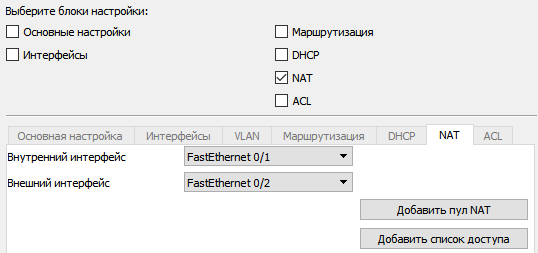
\includegraphics[width=1\linewidth]{pic/nat_settings}
	\caption{NAT}
	\label{fig:nat_settings}
\end{figure}

Укажите внешний и внутренний интерфейс, выбрав нужный из списка доступных.

Для добавления пула NAT, нажмите кнопку \texttt{<<Добавить пул NAT>>} или выберите пункт меню \texttt{Редактирование | Добавить пул NAT}.

Для добавления списка доступа нажмите кнопку \texttt{<<Добавить список доступа>>} или выберите пункт меню \texttt{Редактирование | Добавить список доступа}.

\item 
При выборе блока <<ACL>> становится доступна страница (в соответствии с рисунком \ref{fig:acl_settings}), где можно настроить ACL.

\begin{figure}[th!]
	\centering
	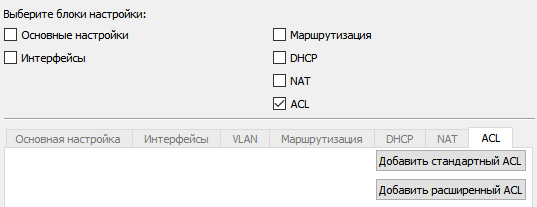
\includegraphics[width=1\linewidth]{pic/acl_settings}
	\caption{ACL}
	\label{fig:acl_settings}
\end{figure}

По умолчанию, ACL отсутствуют. Для добавления ACL, нажмите кнопку \texttt{<<Добавить стандарный ACL>>} или выберите пункт меню \texttt{Редактирование | Добавить стандартный ACL}. 

Для добавления расширенного ACL, нажмите кнопку \texttt{<<Добавить расширенного ACL>>} или выберите пункт меню \texttt{Редактирование | Добавить расширенный ACL}. 
\end{enumerate}

\item Нажмите кнопку <<Сохранить>> для сохранения изменений.

\end{enumerate}

\section{Редактирование шаблона}

Для редактирования шаблона:
\begin{enumerate}
	\item Выберите шаблон (в соответствии с рисунком \ref{fig:edit_template}).
	
	
\begin{figure}[th!]
\centering
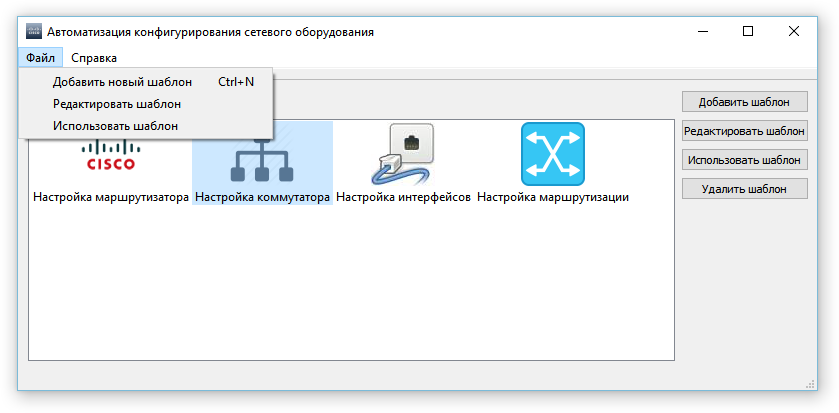
\includegraphics[width=1\linewidth]{pic/edit_template}
\caption{Выделение шаблона}
\label{fig:edit_template}
\end{figure}

	\item Нажмите кнопку \texttt{<<Редактировать шаблон>>} или выберите пункт меню \texttt{Файл | Редактировать шаблон}.
\end{enumerate}
Редактирование осуществляет в окне, аналогичном пункту <<Создание шаблона>> (смотри пункт \ref{section:add_template}).

\section{Использование шаблона}

Для использования шаблона:
\begin{enumerate}
	\item Выберите шаблон (в соответствии с рисунком \ref{fig:edit_template}).
	
	\item Нажмите кнопку \texttt{<<Использовать шаблон>>} или выберите пункт меню \texttt{Файл | Использовать шаблон}.
	
	\item В появившемся окне (пример приведен на рисунке \ref{fig:example}) введите или исправьте установленные по умолчанию значения на необходимые вам.
	
	
\begin{figure}[th!]
\centering
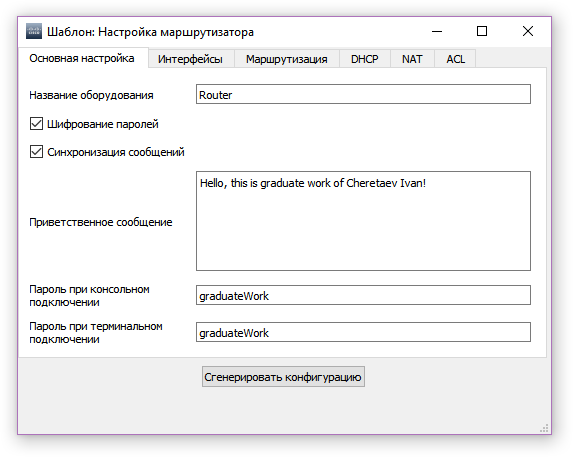
\includegraphics[width=1\linewidth]{pic/example}
\caption{Использование шаблона}
\label{fig:example}
\end{figure}
	
	\item Нажмите кнопку <<Сгенерировать конфигурацию>>.
	
	\item Выберите место сохранения файла и его имя.
\end{enumerate} 

\section{Удаление шаблона}

Для удаления шаблона:
\begin{enumerate}
	\item Выберите шаблон (в соответствии с рисунком \ref{fig:edit_template}).
	
	\item Нажмите кнопку \texttt{<<Удалить шаблон>>} или выберите пункт меню \texttt{Файл | Удалить шаблон}.
	
	\item Подтвердите удаление в появившемся диалоговом окне.
\end{enumerate} 

\section{Справка}

Для запуска справочной системы выберите пункт меню \texttt{Справка | Запуск справки} либо нажмите сочетание клавиш \texttt{Ctrl+H}. Отобразится начальное страница справки, представленная на рисунке \ref{fig:help}.

\begin{figure}[th!]
\centering
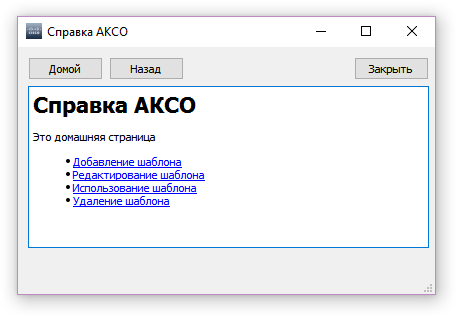
\includegraphics[width=0.8\linewidth]{pic/help}
\caption{Начальная страница справки}
\label{fig:help}
\end{figure}


Для просмотра краткой информации о программе выберите пункт меню \texttt{Справка | О программе}. Результат приведен на рисунке \ref{fig:about}.
\begin{figure}[th!]
\centering
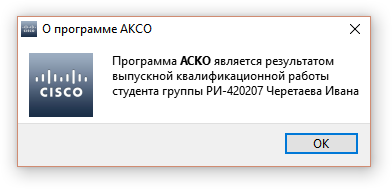
\includegraphics[width=0.8\linewidth]{pic/about}
\caption{Окно <<О программе>>}
\label{fig:about}
\end{figure}
